%! Author = sriadityavedantam
%! Date = 4/7/26

\section{Projective Varieties}

Consider $U = \aa^2\setminus\{(0,0)\}\subset \aa^2$.
It is a fact that there is no natural way to give $U$ the structure of an affine variety.
On the other hand, if we remove a whole curve from an affine variety, the result can still be affine.

\begin{definition}[Localization]
    \[
        \kk[Y]
        \coloneqq \frac{\kk[x_1,\ldots,x_n,y]}{(I(X),\, y - f(x_1,\ldots,x_n))}
        \cong \kk[X]\left[\frac{1}{f}\right].
    \]
    More generally, if $f\in R$, then $R\left[\frac{1}{f}\right]$ denotes the localization of $R$ at $f$.
\end{definition}

\begin{definition}[$\pp^n$]
    \[
        \pp^n
        \coloneqq
        \frac{\{(x_0,\ldots,x_n)\in \kk^{n+1}\setminus\{(0,\ldots,0)\}\}}{\sim},
    \]
    where
    \[
        (x_0,\ldots,x_n)\sim (\lambda x_0,\ldots,\lambda x_n)
    \]
    for every $\lambda\in \kk^\times$.

    Thus the points of $\pp^n$ correspond to lines through the origin in $\aa^{n+1}$.
\end{definition}

\begin{lemma*}{
    \[
        \pp^n = U_0\cup\cdots\cup U_n,
    \]
    where
    \[
        U_i = \{[x_0:\cdots:x_n]\in \pp^n : x_i\neq 0\}\cong \aa^n.
    \]
}
\end{lemma*}

\begin{gather*}
    \pp^1 = \aa^1\cup\{\infty\}.\\
    \pp^n = U_0\cup U_1\cup\cdots\cup U_n,\\
\end{gather*}
with each $U_i\cong \aa^n$.

\[
    \pp^2_{\rr} = \rr^2 \cup \{\text{directions of lines}\} \cong S^2/(z\sim -z).
\]

\begin{figure}[H]
    \centering

    \tikzset{every picture/.style={line width=0.75pt}}

    \colorbox{white}{%
        \color{black}
        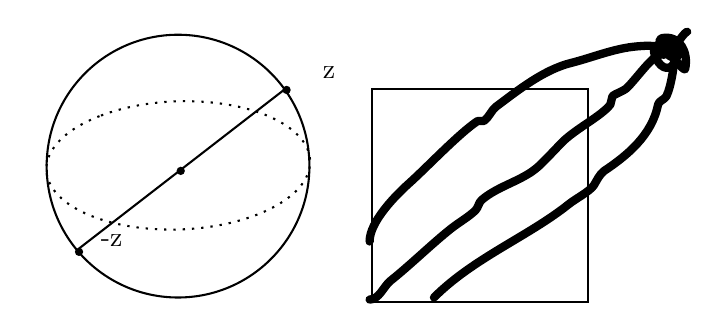
\begin{tikzpicture}[
            x=0.75pt,
            y=0.75pt,
            yscale=-1,
            xscale=1,
            every node/.style={text=black},
            every path/.style={draw=black},
            line width=0.75pt
        ]
            \draw  (174.4,121.3) .. controls (174.4,86.34) and (202.74,58) .. (237.7,58) .. controls (272.66,58) and (301,86.34) .. (301,121.3) .. controls (301,156.26) and (272.66,184.6) .. (237.7,184.6) .. controls (202.74,184.6) and (174.4,156.26) .. (174.4,121.3) -- cycle ;
            \draw  [dash pattern={on 0.84pt off 2.51pt}] (200.59,96.94) .. controls (229.03,86.17) and (268.75,88.2) .. (289.31,101.46) .. controls (309.86,114.73) and (303.47,134.2) .. (275.03,144.97) .. controls (246.59,155.73) and (206.88,153.7) .. (186.32,140.44) .. controls (165.76,127.18) and (172.16,107.7) .. (200.59,96.94) -- cycle ;
            \draw    (190,161) -- (290,83.6) ;
            \draw  [line width=3] [line join = round][line cap = round] (239,123.6) .. controls (239,123.6) and (239,123.6) .. (239,123.6) ;
            \draw  [line width=3] [line join = round][line cap = round] (290,84.6) .. controls (290,84.6) and (290,84.6) .. (290,84.6) ;
            \draw  [line width=3] [line join = round][line cap = round] (190,162.6) .. controls (190,162.6) and (190,162.6) .. (190,162.6) ;

            \draw   (331,84) -- (435,84) -- (435,186.6) -- (331,186.6) -- cycle ;
            \draw  [line width=3] [line join = round][line cap = round] (330,157.6) .. controls (330,148.23) and (342.07,135.8) .. (349,129.6) .. controls (357.52,121.97) and (373.04,105.57) .. (382,99.6) .. controls (382.83,99.05) and (384.17,100.15) .. (385,99.6) .. controls (387.56,97.9) and (388.54,94.44) .. (391,92.6) .. controls (401.8,84.5) and (413.99,74.85) .. (427,71.6) .. controls (437.25,69.04) and (448.07,64.44) .. (459,63.6) .. controls (463.11,63.28) and (471,62.48) .. (471,66.6) ;
            \draw  [line width=3] [line join = round][line cap = round] (330,185.6) .. controls (334.57,185.6) and (336.83,179.14) .. (340,176.6) .. controls (350.05,168.56) and (359.37,159.31) .. (369,151.6) .. controls (372.7,148.64) and (378.02,145.58) .. (381,142.6) .. controls (382.37,141.23) and (382.52,138.86) .. (384,137.6) .. controls (391.65,131.04) and (402.39,128.68) .. (410,122.6) .. controls (413.42,119.86) and (419,113.6) .. (423,109.6) .. controls (429.26,103.34) and (441.9,97.06) .. (446,91.6) .. controls (446.82,90.5) and (446.18,88.7) .. (447,87.6) .. controls (447.61,86.79) and (452.54,85.06) .. (454,83.6) .. controls (458.62,78.98) and (463.43,71.78) .. (469,67.6) .. controls (471.21,65.94) and (476.63,65.35) .. (478,62.6) .. controls (478.67,61.25) and (482.04,56.6) .. (483,56.6) ;
            \draw  [line width=3] [line join = round][line cap = round] (361,184.6) .. controls (380.11,165.49) and (406.51,155.19) .. (426,139.6) .. controls (429.22,137.02) and (436.08,133.48) .. (438,130.6) .. controls (439.15,128.88) and (440.81,125.06) .. (443,123.6) .. controls (454.27,116.09) and (466.06,106.29) .. (469,91.6) .. controls (469.37,89.75) and (472.16,89.29) .. (473,87.6) .. controls (475.31,82.97) and (477,71.47) .. (477,66.6) ;

            \draw  [line width=3] [line join = round][line cap = round] (478,63.6) .. controls (470.83,63.6) and (481.65,76.15) .. (482,74.6) .. controls (483.77,66.63) and (479.7,58.15) .. (471,59.6) .. controls (466.31,60.38) and (475.1,71.5) .. (478,68.6) .. controls (486.67,59.93) and (467.62,60.85) .. (467,64.6) .. controls (466.45,67.88) and (470.41,75.89) .. (475,73.6) .. controls (476.96,72.62) and (480.98,64.04) .. (477,63.6) .. controls (467.51,62.55) and (463.85,67.6) .. (472,67.6) ;

            \draw (199,153) node [anchor=north west][inner sep=0.75pt] {\mbox{-}z};
            \draw (306,72) node [anchor=north west][inner sep=0.75pt] {z};
        \end{tikzpicture}
    }
\end{figure}

Note that for $\pp^2_{\c}$, we have $\cdim(\pp^2_{\c}) = 2$, while $\rdim(\pp^2_{\c}) = 4$.

\begin{lemma*}{
    If $X$ is a complex algebraic variety with $\cdim(X) = d$, then its underlying real manifold, when smooth, has real dimension $2d$.
}
\end{lemma*}

Think of the following coordinates in $\aa$ and in $\pp$.
The function $x_0$ makes sense on $\aa^{n+1}$, but not on $\pp^n$.
However, the condition $x_0 = 0$ does make sense on $\pp^n$.

\begin{definition}[Zero Sets in Projective Space]
    If $p$ is a homogeneous polynomial, then
    \[
        Z_+(p)
    \]
    denotes its well-defined zero set in projective space.
\end{definition}

\begin{definition}[Homogeneous]
    A polynomial is homogeneous if all of its monomials have the same degree.
\end{definition}

\begin{definition}[Graded Rings]
    \[
        R = \bigoplus_{d=0}^{\infty} R_d = \kk[x_0,\ldots,x_n],
    \]
    where each $R_d$ is the space of homogeneous polynomials of degree $d$, and
    \[
        R_a\cdot R_b \subseteq R_{a+b}.
    \]
\end{definition}

\begin{definition}[Dehomogenization]
    Dehomogenization is the process of passing from homogeneous coordinates to affine coordinates, for instance on the chart $x_0\neq 0$:
    \[
        (x_0,\ldots,x_n)\mapsto \left(\frac{x_1}{x_0},\ldots,\frac{x_n}{x_0}\right).
    \]
\end{definition}

\begin{lemma*}{
    If $p$ is homogeneous of degree $d$, then its dehomogenization on any standard affine chart has degree at most $d$.
}
\end{lemma*}